\section{Bevezetés}
	1986-ban Binning demonstrálta az atomerő mikroszkóp (AFM) ötletét \cite{Binnig1986}, ami mára 
	a nanotechnológia egyik legfontosabb eszköze lett. Felhasználható képalkotásra, nanolitográfiára és 
	adott anyag alakítására \cite{Vasic2013}.
	Az AFM apparátusa az adott minta felülete és a felette pásztázó kantilever végére erősített tű 
	kölcsönhatásának vizsgálatát végzi. (lásd \ref{fig:tip-sample}. ábra)
	A felület és a tű közötti domináns kölcsönhatás határozza meg, hogy az anyag melyik fizikai
	mennyiségét kaphatjuk meg.
	\begin{figure}[H]
		\centering
		\subfloat[Az AFM apparátusa]{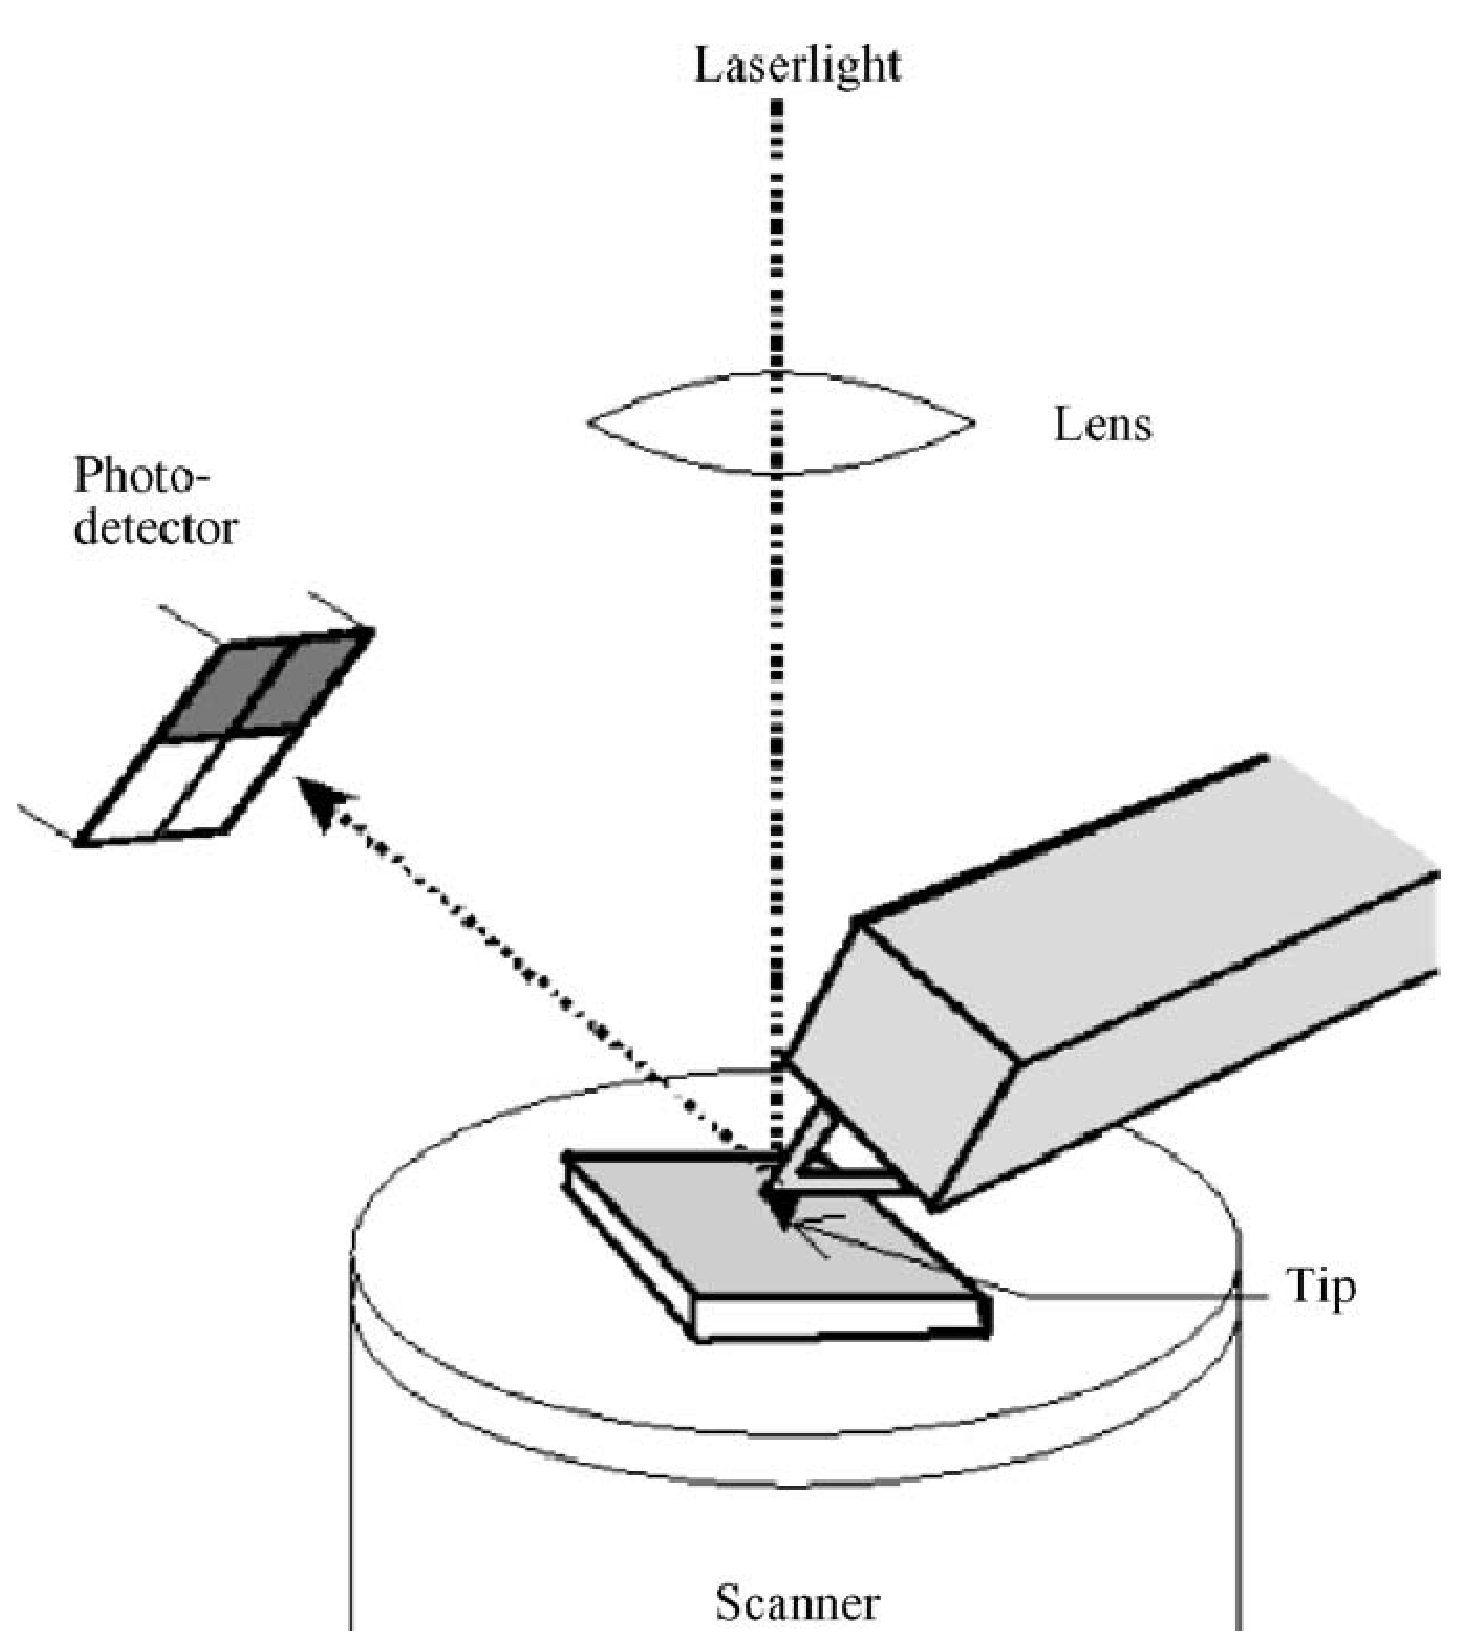
\includegraphics[width=0.45\columnwidth]{kepek/eps/AFM.eps}%
		\label{fig:afm}}
		\hfil
		\subfloat[A tű és minta modellje]{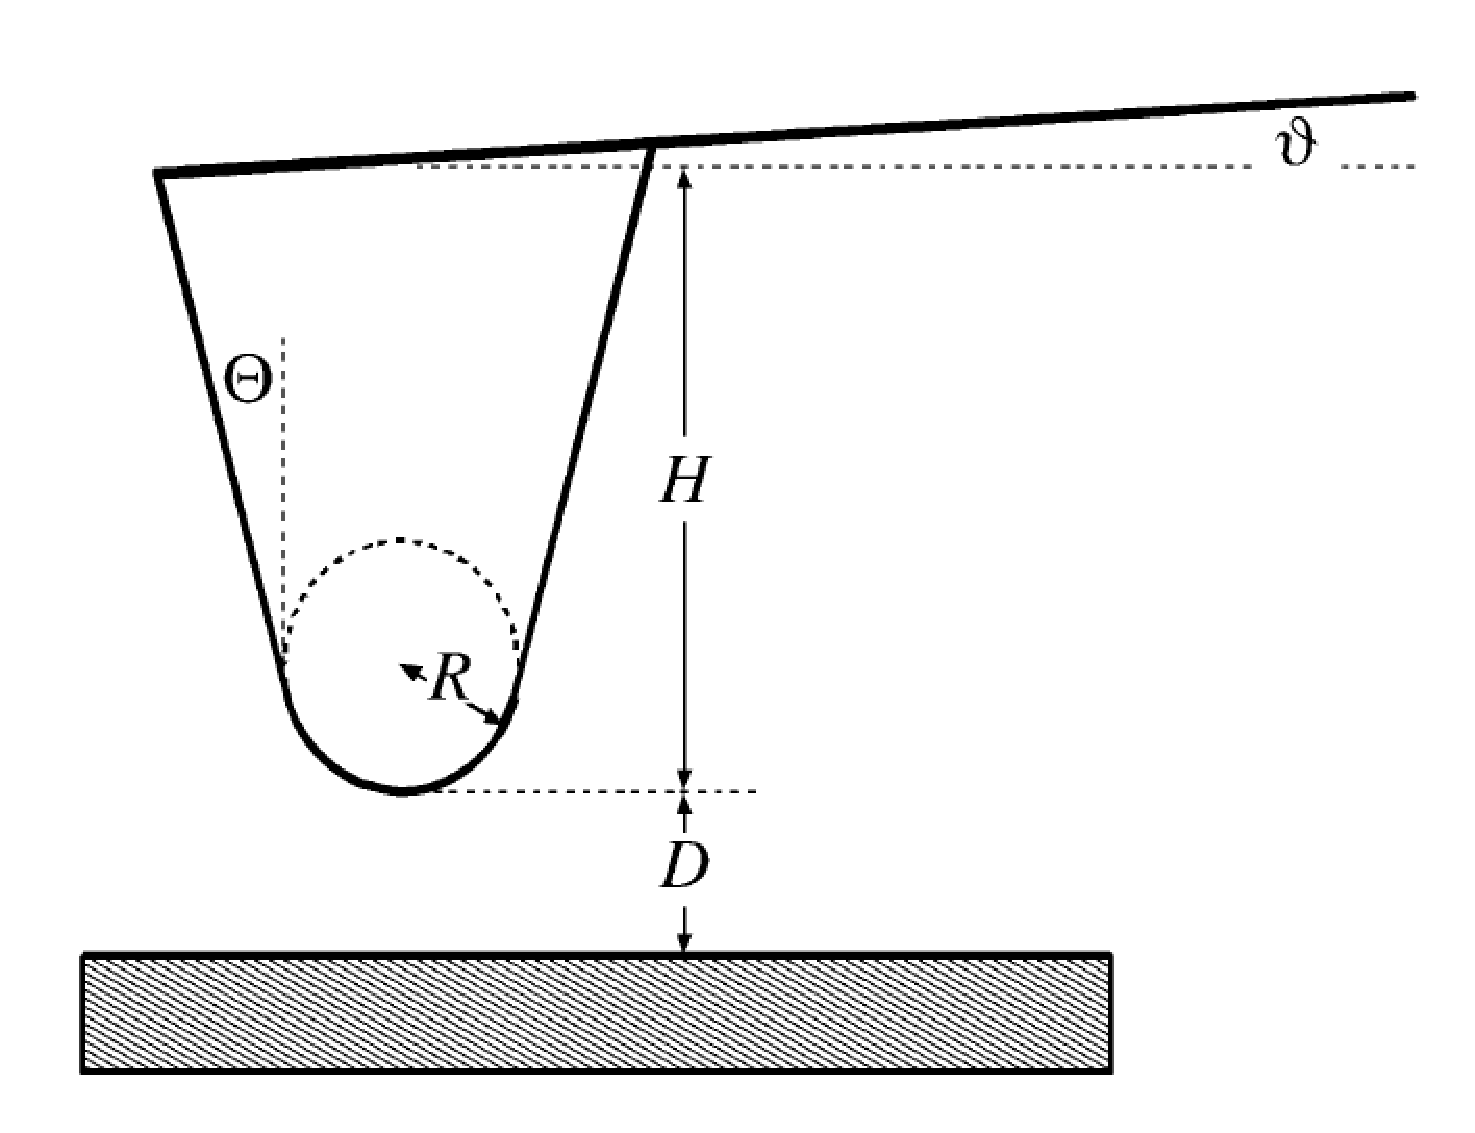
\includegraphics[width=0.45\columnwidth]{kepek/eps/tip-sample.eps}%
		\label{fig:tip-sample}}
		\caption{\scriptsize Az AFM apparátusa látható az (a) ábrán. A lázernyaláb
		a kantilever felületéről tükröződve egy fotódetektorra irányul. A tű pozícióját ez alapján nagy pontossággal ismerjük. A
		(b) ábrán a minta és a felette lévő tű modellje látható a kapacitás analitikus számításához.
		A tű $R$ sugarú $H$ magasságú és $D$ távolságra van a mintától. (Forrás: \cite{Butt20051})}
		\label{fig_sim}
	\end{figure}
	Az AFM felhasználása kontakt illetve kopogtató üzemmódú lehet. A kontakt mód során a
	felületen végighúzzuk a tűt és mérjük a $z$ irányű elmozdulását. Így képesek vagyunk a minta
	felületén lévő atomok elrendezéséről magasságtérkép adni.
	Kopogtató mód \cite{Martin1987} során a tűt elemeljük a mintától és $f$ frekvenciával rezegtetjük.
	A letapogatás során az  átlagos minta-tű távolságot a kontakt módú magasságtérkép felhasználásával
	konstans értéken tartjuk.
	A kantilever dinamikáját ismerve a rezegtetés frekvenciájának eltéréséből
	számítható a tűre ható erő. Ezen erő nagyságát két tényező befolyásolja:
	\begin{enumerate}[a)]
		\item a minta és a tű közötti feszültség,
		\item a minta felületi töltéssűrűség eloszlása.
	\end{enumerate}
	A cikkben a felületi töltéssűrűség mérését tekintjük célnak.
	A \cite{Butt20051} szerint az erő a) komponensét a minta és a tű közötti kapacitásból a
	(\ref{eq:cap_force}) szerint származtathatjuk.
	\begin{equation}
	\label{eq:cap_force}
	F_{s} = -\frac{\ud E}{\ud D} = -\frac{\ud (CV^2 /2)}{\ud D} = -\frac12 \frac{\ud C}{\ud D} V^2
	\end{equation}
	Ha a minta pásztázása során ezen a) erőkomponens konstansnak mondható, tehát a felületi
	érdesség kicsi, akkor a töltéssűrűg mérésében állandó hibát okozva eliminálható.
	Az (\ref{eq:cap_force}) számításában a kritikus elem a kapacitás értéke, amit numerikus számítás
	mellőzése esetén a \cite{Hudlet1998} szerinti analitikus eredményt használhatjuk fel.
	A tű formályát a (\ref{fig:tip-sample} ábra) szerintinek veszi és a mintát sík felületünek
	feltételezi.
	Ezen utóbbi feltételezés legtöbb esetben helyénvaló, viszont a minta nagyfokú érdessége és a
	tű egyedi formálya esetén érvényét veszti. Ilyen esetben a kapacitás értéke mintáról
	mintára változik és állandó hiba helyett, a mérést zajként terheli.
	A kapacitás numerikus szimulációjával ezen zajt is ki lehet küszöbölni.
	Persze ezen szimulációt minden egyes mérési pontban el kell végezni, aminek a kivitelezése
	csak multiprocesszoros környezetben lehetséges elfogadható idő alatt.
	
\section{A feladat}
	A minta egy fémezett felület, aminek magasságtérképét mérések eredményeként ismerjük
	adott pontossággal.
	A mérések egy négyzetes háló felett történtek, amelynek a háló mindkét irányban
	$\delta_x = \delta_y = 120 nm$ azonos felbontása, illetve a magasság $\delta_z = 20nm$ felbontása
	volt.
	A töltéssűrűség méréséhez szükséges második pásztázás során a tűt felemeljük és a mintához képest
	$V_{tu}$ potenciálra kapcsoljuk. Ezután a fémezett felülettől mindig azonos távolságra tartjuk és ezen 
	hosszú hegyes tűre ható erőt mérjük.
	\noindent
	\begin{center}
	Végső cél olyan szimulátor építése, amelynek segítségével közel valós időben 
	lehetséges felületmérés alapján a felületi töltéseloszlásról korrigált/pontosabb információt
	kapni.
	\end{center}
	
	A cikkben felhasznált mérési eredmény (\ref{fig:felulet}. ábra) egy
	$512\times512$ méretű szürkeárnyalatos *.tiff állomány, amely értékei $0-255$-ig terjed.
	
	\begin{figure}[!h]
		\centering
		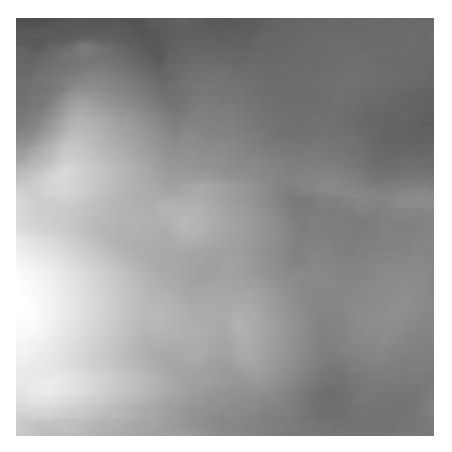
\includegraphics[width=0.45\columnwidth]{kepek/eps/afm200.eps}
		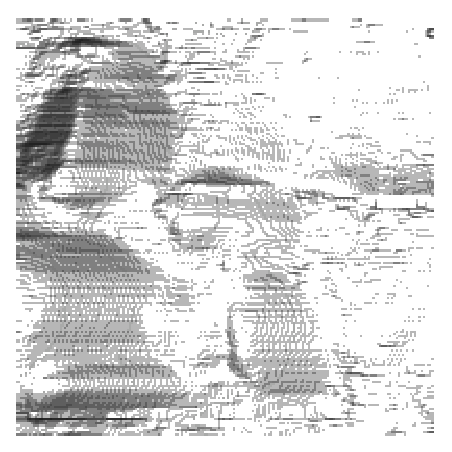
\includegraphics[width=0.45\columnwidth]{kepek/eps/efm200.eps}
		\caption{\scriptsize Méréssel kapott felület (balra) és szimulációval kapott töltéstérkép}
		\label{fig:felulet}
	\end{figure}
	
	
	
\section{Szimuláció} 
\subsection{Fizikai probléma matematikai formalizálása}
	
	A megoldandó feladat egy elektrosztatikus feladat.
	A minta és a tű közötti térben nincsenek töltések, így itt a Poisson egyenlet helyett a
	Laplace-egyenlet \eqref{eq:laplace} érvényes.
	\begin{equation}\label{eq:laplace}
		\Delta V(x,y,z) = 0 
	\end{equation}
	Az egyenletet későbbiekben részletezett (\ref{sec:felepites}) megfontolások végett egy redukált
	3D-s téren oldjuk meg.
	Ezen 3D-s térre egy inhomogén ponthálót illesztünk, amelynek vízszintesen $d_x = d_y$,
	függőlegesen $d_z$ a felbontása. A függőleges felbontás megegyezik a használt AFM apparátus
	felbontásával $d_z = \delta_z$.
	Az így kapott térbeli háló minden pontjához hozzárendeljük az $V_{i,j,k} \simeq V(id_x,jd_y,kd_z)$
	potenciált.
	Dirichlet határfeltételek a felület fémezése, amely zérus potenciálú és az adott ($V_{tu}$)
	potenciálú  tű fémes felülete.
	A térnek a minta felületétől különböző határfelületén homogén Neumann feltételt alkalmazunk
	a szimmetriák (végtelen tér) és a töltésmentesség miatt.
	
	Az így adódó lineáris egyenletrendszer megoldására lehetséges direkt és iteratív megoldó
	algoritmusokat alkalmazni.
	%($1\leq i\leq i_{max}$, $1\leq j\leq j_{max}$, $1\leq k\leq k_{max}$). 
% 	Az alkalmazott interpoláció során a függőleges irányú felbontást is figyelembe véve 
	A párhuzamosítási szándékok miatt az iteratív megoldást választottuk, mivel a multiprocesszoros
	környezetek tipikusan kevés fajlagos-memóriával \footnote{Fajlagos alatt az egy szimulációra jutó
	memóriát értem. (Természetesen ezen szimulációk egyszerre futnak, így a fajlagos-memória
	akkumulálódik.)} rendelkeznek.
	Ekkor nem teljesen pontos megoldást kapunk, azonban gyorsabban juthatunk el a kívánt eredményhez.
	A számítási pontosság növelhető az iterációt leállító konvergencia követelmény keményebb
	megszabásával, ami persze több iterációt jelent.
	
	Az iteratív megoldás során a megoldás aktuális értékének kiszámításához az előző megoldásból indulunk ki.
	A \eqref{eq:laplace} egyenletben szereplő deriválást az elsőrendű Taylor közelítés alkalmazásával a
	\eqref{eq:it} 6-pontos sémát kapjuk.
	\begin{multline} \label{eq:it} 
		V_{ijk}^{n+1} = \\ \Delta_1 \cdot \left(V_{i-1,j,k}^n+V_{i+1,j,k}^n
		+V_{i,j-1,k}^n+V_{i,j+1,k}^n\right)+ \\
						\Delta_2 \cdot \left(V_{i,j,k-1}^n+V_{i,j,k+1}^n\right)
	\end{multline}
	ahol $V_{i,j,k}^n$ az az $n$-dik iterációs lépésben az $i,j,k$ indexü
	pontban mérhető potenciált jelöli, $\Delta_1$ a vízszintes felbontásból,
	$\Delta_2$ a függőleges felbontásból adódó állandó.
	%Az iterációs eljárás előnye, hogy implementációja egyszerűbb és a
	%\eqref{eq:2} szerinti ``simítás'' gyorsabb, mint a direkt megoldás.
	%Az iterációs eljárás előnye, hogy memóriaigénye kicsi a direkt megoldás során
	% adódó egyenletmegoldáshoz képest.
	%Hátránya hogy nem ad pontos választ egy lépésben.
	
% 	\begin{figure}[!ht]
% 		\centering
% 		\psfrag{ijk}{$(i,j,k)$}
% 		\psfrag{imjk}{$(i-1,j,k)$} 
% 		\psfrag{ipjk}{$(i+1,j,k)$}
% 		\psfrag{ijmk}{$(i,j-1,k)$} 
% 		\psfrag{ijpk}{$(i,j+1,k)$}
% 		\psfrag{d1}{$k_x$} 
% 		\psfrag{d2}{$k_y$} 
% 		\psfrag{d3}{$k_z$} 
% 		\psfrag{ijkm}{$(i,j,k-1)$} 
% 		\psfrag{ijkp}{$(i,j,k+1)$} 
% 		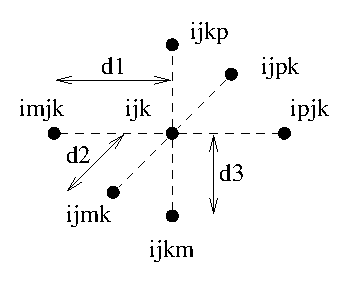
\includegraphics[width=0.95\columnwidth]{kepek/eps/sema.eps}
% 		\caption{\scriptsize Diszkretizálás során alkalmazott felosztás} 
% 	\end{figure}

	
% 	fi(idx,idy,idz) = KK1*(fip(idx-1,idy,idz)+fip(idx+1,idy,idz)+fip(idx,idy-1,idz)+fip(idx,idy+1,idz))+...
%               KK2*(fip(idx,idy,idz-1)+fip(idx,idy,idz+1))

\subsection{Szimuláció felépítése} \label{sec:felepites}
	
	A felületmérés során a vízszintes felbontás joval kissebb, mint a függőleges felbontás
	$d_x=d_y \gg d_z$. A Coulomb-kölcsönhatás a távolság négyzetével fordítottan arányos,
	így az előbb említettek értelmében egy mérési pont szomszédjait, pontosabban egy redukált
	környezetét szükséges csupán szimulálni. (Másképpen megfogalmazva a vízszintes mérési pontok
	távolsága jóval nagyobb mint a Coulomb-kölcsönhatás effektív távolsága.) Ezzel az elhanyagolással
	már numerikusan kezelhető bonyulultságú problémára jutunk.
	
	Ezen módon egy mért pont $3\times3$-as környezetét vesszük figyelembe,
	a középső pont felett lévő elektródát (tűt) feltételezve.
	A szimulációs tér alsó felületét a mért magassági $3\times 3$ mintákból kell meghatároznunk.
	Mivel ezen pontokra úgy is tekinthetünk, mint a minta magasság-függvényének a mintavételezésével
	kapott mintáira, így a küzbünső pontokat interpolációval/ideális aluláteresztéssel kaphatjuk meg.
	Az interpoláció $N_{ip}$ faktorával \footnote{$N_{ip}$-szeresére növeljük a pontok számát.}
	lehetséges a szimulációs tér vízszintes felbontását $d_x=d_y = \delta_x / N_{ip}$ megkapni.

	A szimulációk során a felület magasságának mérési adatait már ismertnek feltételezzük.
	A teljes magasságtérkép pontjait külön-külön vizsgáljuk.
	Egyetlen pontban a mérési eredmény kiszámításának lépései az alábbiak :
	
	\begin{enumerate}
		\item A pont körüli felület $3\times3$-as mérési részének megállapítása,
		\item Közbenső (virtuális) mérési pontokkal a belső felbontás növelése
		interpolációval,
		\item Szimulálandó tér méretének számítása,
		\item Direkt/iteratív megoldó algoritmussal a tér meghatározása, 
				a tűre ható erő számítása illetve a tű alatti töltésmennyiség számítása,
		\item Adatok mentése.
	\end{enumerate}
	

	